\section{Additive forecasting: interpretation and research record}
\label{app:utility}

\subsection{Oracle residual structure and finite correction}
\label{app:utility-projection}
Condition on development data and the fitted maps $f_0$ and $\Gamma$.
For $e=Y-f_0(X)$, suppose $\E\|e\|_2^2<\infty$, let $Z=\Gamma(X)$,
and put $q^*(Z)=\E[e\mid Z]$. For any square-integrable $q(Z)$,
conditional expectation makes the cross term zero, giving
\[
 \E\|e-q(Z)\|_2^2
 =\E\|e-q^*(Z)\|_2^2+\E\|q^*(Z)-q(Z)\|_2^2.
\]
Taking $q=0$ and then the infimum over $q$ proves
Equation~\eqref{eq:utility-oracle}. This standard projection argument
establishes an oracle notion of residual predictive structure, not its
estimability with a finite sample, a specified ridge head, or a given
computation budget. The conditional distribution and expectations are
those of the evaluation law given the frozen fitted state. A deterministic
feature of $X$ cannot create new information absent from that history;
the comparison is with the particular baseline $f_0$, not with the
unrestricted raw-history Bayes predictor.

\subsection{Residual alignment for a frozen correction}
\label{app:utility-alignment}
This subsection records a standard squared-loss calculation; it is not
claimed as a new general learning principle. Condition on development data
and all random choices used to fit a baseline $f_0$ and a correction $q$.
Suppose $\E\|Y-f_0(X)\|_2^2<\infty$ and
$\E\|q(X)\|_2^2<\infty$. Write
\[
 A=\E\langle Y-f_0(X),q(X)\rangle,\qquad
 B=\E\|q(X)\|_2^2.
\]
Expanding the squared norm yields
\[
 \E\|Y-f_0(X)-\gamma q(X)\|_2^2
 =R(f_0)-2\gamma A+\gamma^2B.
\]
If $B=0$, then $q(X)=0$ almost surely, so $A=0$ and the correction changes
no population forecast. If $B>0$, minimization over $\gamma\in[0,1]$ gives
$\gamma^*=\clip(A/B,0,1)$. A positive weight improves risk precisely when
$A>0$ and $0<\gamma<2A/B$. Thus a useful correction must align with the
baseline's residual under the evaluation law, with its scale controlled.
The same identity holds for a loss averaged across target coordinates
after both $A$ and $B$ are divided by their common coordinate count.

This oracle calculation uses population quantities unavailable to the
fitted selector. Empirical residual fitting, regularization, and validation
introduce estimation and selection effects. Inclusion of $\gamma=0$ makes
the original forecast feasible; it does not imply that the selected test
forecast is no worse. In particular, correlation with training residuals
does not prove positive $A$ on a new episode or source.

\subsection{Distinction from representation-class certificates}
\label{app:utility-scope}
The empirical difference in Equation~\eqref{eq:utility-delta} compares two
frozen fitted forecasts. The certificate manuscript instead studies the
infimum of risk over a declared representation--decoder class, and can
exclude that entire class under its assumptions
\citep{Anonymous2026Certificates}. The additive study does not transfer
such a class-level guarantee to its forecasts. A certificate for a residual
component would not automatically certify the complete additive forecast;
the baseline and correction together would have to satisfy the declared
representation, metric, and sensitivity constraint. Neither mean test
differences nor a zero-correction option establishes necessity of the
additional features among all possible decoders.

\subsection{Extension protocol and source roster}
\label{app:utility-protocol}

The executable configuration and protocol for this extension are stored
in \path{extensions/forecasting_utility}. They define a distinct study
from the original controlled, natural-source, and scaling studies. The
execution freeze hashes the configuration, protocol, source and dependency
files, archive metadata, and training-prefix-selected roster before full
model evaluation. Its purpose is to make subsequent deviations and
recomputation auditable; it is not external review or registration.

\begin{table}[ht]
\centering\small\setlength{\tabcolsep}{4pt}
\caption{Additional archive collections and the fixed hash-selected roster.
Each selected series is evaluated at $M=16$ and $64$. $L$ is history
length, $H$ is the number of consecutive direct target steps, and $p$ is
the declared seasonal period. The Solar collection has simulation
provenance. Source record DOIs, byte hashes, and licenses are retained in
the artifact.}
\label{tab:utility-roster}
\begin{tabular}{llrrrl}
\toprule
Collection & Frequency & $L$ & $H$ & $p$ & Selected series \\
\midrule
Weather & Daily & 28 & 7 & 7 & T1476, T1967, T416 \\
Solar Weekly & Weekly & 6 & 2 & 52 & T88, T94, T8 \\
COVID-19 Deaths & Daily & 28 & 7 & 7 & T42, T146, T96 \\
Car Parts, missing & Monthly & 6 & 2 & 12 & T1324, T2368, T857 \\
\bottomrule
\end{tabular}
\end{table}

Weather contains daily Australian weather-station variables, COVID-19
Deaths contains the archived Johns Hopkins death-count series, and Car
Parts contains intermittent monthly sales extracted from the
\texttt{expsmooth} collection. The exact Monash records are
10.5281/zenodo.4654822, 10.5281/zenodo.4656009, and
10.5281/zenodo.4656022, respectively. Solar Weekly is record
10.5281/zenodo.4656151 and contains aggregated simulated NREL production
series. All four downloaded records declare CC BY 4.0. The use of a
historical public snapshot does not establish real-time revision-aware
evaluation; upstream release vintages and the original producers'
measurement pipelines are not reconstructed here.

Training-prefix eligibility requires at least 16 complete available
training windows and a positive finite error scale. Hash ordering uses
the fixed salt \texttt{forecasting-utility-natural-v1} and the source and
series identifiers. Complete contexts and targets are required; no
future-aware missing-value filling is applied. This defines an
available-window forecasting estimand. The scaling denominator uses the
uncapped initial training prefix and is unchanged by the selected
pretest refit. Periods are stated in Table~\ref{tab:utility-roster}; when
the seasonal-difference mean square is unavailable or zero, the
first-difference mean square is used. This scale is not a fitted
baseline's test error.

The naive forecast uses the seasonal observation when available and the
last available observation otherwise; synthetic episodes use persistence.
The seasonal lag may extend beyond the finite context supplied to the
learned models, particularly for weekly Solar and monthly Car Parts.
Thus this practical control shares their targets and forecast origins,
but not necessarily their identical finite-history information set;
every observation it accesses is available at or before the forecast origin.
The practical nonlinear control fits an independent histogram-gradient
regressor per target coordinate, with 100 iterations, at most 15 leaves,
$L_2$ penalty 0.01, and early stopping disabled. It receives the same
raw histories and split origins, without a separate hyperparameter search.
This is one fixed practical control, not a comprehensive comparison with
modern neural, pretrained, probabilistic, or multivariate forecasters.

For every model, preprocessing is fitted on the permitted fitting inputs
only. An additive correction first receives residuals from the selected
raw predictor on those same fitting rows. A natural-data pretest refit
rebuilds both the raw predictor and the correction using the chosen
settings; thus the final raw component differs from the validation-stage
fit but is again held fixed while its correction is fitted. Synthetic
fits retain training-only inputs. A final zero-weight correction bypasses
geometry at prediction time, but its already incurred selection costs
remain charged. Additional candidate searches are therefore observable
costs even when the deployed forecast equals the raw baseline.
The synthetic zero-weight fit retains its searched correction bank in
memory, because the selected training-only object is retained. The natural
zero-weight refit omits that bank. Reported serialized bytes describe this
actual stored state, not the smallest equivalent deployable model;
neither case evaluates the correction during a zero-weight prediction.

Full validation-candidate records, chosen penalties and mixing weights,
warnings, split origins, saved forecasts, and wall/CPU timing components
are retained. Saved test forecasts permit independent reconstruction of
both episode-level synthetic losses and original-unit and scaled
archive-source losses. A task or method failure is recorded with its
exception and does not silently select a replacement source, seed, or
model. The completeness audit distinguishes requested configurations,
successful outputs, and failures before producing the manuscript assets.

\subsection{Complete controlled comparisons and source-level results}
\label{app:utility-results}

Table~\ref{tab:utility-failures} retains every incomplete configuration.
The failed series is also retained in the original roster and window
table. Full-roster geometry and policy losses remain undefined. The
separate reporting amendment creates a post-hoc matched-success
diagnostic on 22 configurations and 11 series, without changing a fitted
model, source, or validation rule. The archive displays below use that
diagnostic support unless explicitly marked as full-roster coverage.

% Generated from the audited forecasting-utility extension; no model fitting.
\begin{table}[!htbp]
\centering\small\setlength{\tabcolsep}{4pt}
\caption{Every incomplete configuration in the frozen execution. The shared bank requests eight nonempty groups but these training inputs have only seven distinct histories. Concatenated KAHM and additive KAHM, affine, and locality each fail; both dependent policies have no decision. The specified method reports a fitting failure when the requested groups cannot be formed. The four baseline forecasts are retained.}
\label{tab:utility-failures}
\begin{tabular}{llrrrrr}
\toprule
Source & Series & $M$ & Train rows & Distinct & Failed fits & Failed policies \\
\midrule
Car Parts & T1324 & 16 & 23 & 7 & 4 & 2 \\
Car Parts & T1324 & 64 & 23 & 7 & 4 & 2 \\
\bottomrule
\end{tabular}
\end{table}


The new controlled means in Table~\ref{tab:utility-synthetic} are
supplemented by every practical control and fixed policy in
Table~\ref{tab:utility-synthetic-controls}. Table~\ref{tab:utility-intervals}
gives all 24 primary interval endpoints. The raw and concatenated
contrasts form this extension's family only; intervals are not
retroactively pooled with the original studies' inference.

% Generated from the audited forecasting-utility extension; no model fitting.
\begin{table}[!htbp]
\centering\small\setlength{\tabcolsep}{4pt}
\caption{Remaining controls and declared policies in the same new synthetic factorial. Mean MSE is multiplied by $10^3$. The two policies use the fixed 5\% validation margin; their test losses are descriptive.}
\label{tab:utility-synthetic-controls}
\begin{tabular}{lrrrrrrr}
\toprule
Law & $N$ & $M$ & Raw ridge & Persistence & Boosting & KAHM rule & Geometry rule \\
\midrule
Nonlinear AR & 32 & 16 & 5.4248 & 8.8523 & 5.6510 & 4.8163 & 4.8163 \\
Nonlinear AR & 32 & 64 & 5.4248 & 8.8523 & 5.6510 & 5.0133 & 5.0133 \\
Nonlinear AR & 128 & 16 & 5.3733 & 8.8523 & 4.8297 & 4.6648 & 4.6570 \\
Nonlinear AR & 128 & 64 & 5.3733 & 8.8523 & 4.8297 & 4.4806 & 4.4806 \\
Van der Pol & 32 & 16 & 61.0069 & 290.7804 & 3.9407 & 15.6100 & 12.8539 \\
Van der Pol & 32 & 64 & 61.0069 & 290.7804 & 3.9407 & 8.2892 & 7.9561 \\
Van der Pol & 128 & 16 & 60.8383 & 290.7804 & 1.4755 & 14.4955 & 11.5577 \\
Van der Pol & 128 & 64 & 60.8383 & 290.7804 & 1.4755 & 7.4507 & 7.0588 \\
Duffing & 32 & 16 & 15.3586 & 38.7289 & 7.4754 & 6.6748 & 5.2717 \\
Duffing & 32 & 64 & 15.3586 & 38.7289 & 7.4754 & 5.3159 & 4.7580 \\
Duffing & 128 & 16 & 14.8690 & 38.7289 & 4.7537 & 5.8873 & 4.5908 \\
Duffing & 128 & 64 & 14.8690 & 38.7289 & 4.7537 & 4.3081 & 3.6958 \\
\bottomrule
\end{tabular}
\end{table}

% Generated from the audited forecasting-utility extension; no model fitting.
\begin{table}[!htbp]
\centering\small\setlength{\tabcolsep}{4pt}
\caption{Every primary new synthetic contrast. Differences and interval endpoints are multiplied by $10^3$; positive differences favor additive KAHM. The 24 intervals form their own 95\% Bonferroni paired Student family over 12 complete repetitions. The normality approximation is not a distribution-free guarantee or joint coverage claim with earlier studies.}
\label{tab:utility-intervals}
\begin{tabular}{lrrlrr}
\toprule
Law & $N$ & $M$ & Control & $\Delta$ & Simultaneous interval \\
\midrule
Nonlinear AR & 32 & 16 & Raw RBF & 0.1190 & [-0.0325, 0.2706] \\
Nonlinear AR & 32 & 16 & Concat. & 0.2326 & [0.0750, 0.3902] \\
Nonlinear AR & 32 & 64 & Raw RBF & -0.0024 & [-0.0155, 0.0107] \\
Nonlinear AR & 32 & 64 & Concat. & 0.3230 & [0.0983, 0.5478] \\
Nonlinear AR & 128 & 16 & Raw RBF & 0.0947 & [-0.0443, 0.2337] \\
Nonlinear AR & 128 & 16 & Concat. & 0.0891 & [0.0195, 0.1587] \\
Nonlinear AR & 128 & 64 & Raw RBF & 0.0000 & [-0.0051, 0.0051] \\
Nonlinear AR & 128 & 64 & Concat. & 0.2201 & [0.1437, 0.2965] \\
Van der Pol & 32 & 16 & Raw RBF & 6.4813 & [3.8242, 9.1385] \\
Van der Pol & 32 & 16 & Concat. & -8.5175 & [-13.2045, -3.8305] \\
Van der Pol & 32 & 64 & Raw RBF & 0.9173 & [0.3991, 1.4356] \\
Van der Pol & 32 & 64 & Concat. & -5.6375 & [-6.7666, -4.5083] \\
Van der Pol & 128 & 16 & Raw RBF & 6.0508 & [4.0580, 8.0435] \\
Van der Pol & 128 & 16 & Concat. & -6.9265 & [-11.4856, -2.3674] \\
Van der Pol & 128 & 64 & Raw RBF & 0.9524 & [0.6890, 1.2159] \\
Van der Pol & 128 & 64 & Concat. & -5.0420 & [-5.7154, -4.3685] \\
Duffing & 32 & 16 & Raw RBF & 0.6926 & [-0.0149, 1.4001] \\
Duffing & 32 & 16 & Concat. & 1.9464 & [1.1163, 2.7766] \\
Duffing & 32 & 64 & Raw RBF & 0.0200 & [-0.0226, 0.0625] \\
Duffing & 32 & 64 & Concat. & -0.2612 & [-1.0430, 0.5206] \\
Duffing & 128 & 16 & Raw RBF & 0.8065 & [0.3672, 1.2458] \\
Duffing & 128 & 16 & Concat. & 1.7380 & [0.9065, 2.5694] \\
Duffing & 128 & 64 & Raw RBF & 0.0548 & [-0.0243, 0.1339] \\
Duffing & 128 & 64 & Concat. & -0.2138 & [-0.5053, 0.0777] \\
\bottomrule
\end{tabular}
\end{table}

\FloatBarrier

The new matched-success archive diagnostic is resolved by source in
Table~\ref{tab:utility-archive-sources}. Window counts and effective
decoder sizes appear in Tables~\ref{tab:utility-windows}
and~\ref{tab:utility-decoder-sizes}. Counts are shared across methods,
and requested Nystr\"om sizes can be capped by short fitting segments.
The selected weights and policy decisions in
Tables~\ref{tab:utility-gamma} and~\ref{tab:utility-policy-choices}
describe related task configurations, not independent draws of a
universal adoption probability. Table~\ref{tab:utility-leave-one}
retains every leave-one-source-out re-aggregation without selecting
the most favorable subset.

% Generated from the audited forecasting-utility extension; no model fitting.
\begin{table}[!htbp]
\centering\small\setlength{\tabcolsep}{4pt}
\caption{Post-hoc matched-success scaled MSE by new archive source, averaging capacities within series and then series. The 22 configurations contain three Weather, three Solar, three COVID, and two Car Parts series; the failed Car Parts series is excluded only from this diagnostic. Solar Weekly has simulation provenance. All procedures and both frozen policies are shown.}
\label{tab:utility-archive-sources}
\begin{tabular}{lrrrr}
\toprule
Procedure & Weather & Solar & COVID & Car Parts \\
\midrule
Raw ridge & 0.3363 & 2.1992 & 0.6404 & 0.2106 \\
Raw RBF & 0.3181 & 3.0358 & 33.1371 & 0.2010 \\
Concatenated KAHM & 0.3178 & 2.9745 & 1.3490 & 0.2031 \\
Additive KAHM & 0.3213 & 3.0358 & 33.0164 & 0.2038 \\
Additive affine & 0.3189 & 3.0358 & 33.7662 & 0.2038 \\
Additive locality & 0.3189 & 2.9891 & 34.3905 & 0.5510 \\
Persistence / seasonal naive & 0.5793 & 1.4511 & 2.4268 & 0.3676 \\
Histogram gradient boosting & 0.4482 & 1.9788 & 38.5859 & 0.2567 \\
KAHM 5\% rule & 0.3213 & 3.0358 & 33.4246 & 0.2024 \\
All-geometry 5\% rule & 0.3192 & 2.9891 & 33.1917 & 0.5496 \\
\bottomrule
\end{tabular}
\end{table}

% Generated from the audited forecasting-utility extension; no model fitting.
\begin{table}[!htbp]
\centering\small\setlength{\tabcolsep}{4pt}
\caption{Exact available-window counts for all twelve originally selected series, including Car Parts T1324 whose geometric fits fail, after the fixed caps. Inputs and targets are shared by the two capacities and every procedure. Initial training observations set the scale; refit windows stop before the reserved test boundary. These windows are related observations, not independent source replications.}
\label{tab:utility-windows}
\begin{tabular}{llrrrrrl}
\toprule
Source & Series & Length & Train & Valid. & Refit & Test & Scale \\
\midrule
Weather & T1476 & 14262 & 512 & 64 & 512 & 64 & Seasonal \\
Weather & T1967 & 6810 & 512 & 64 & 512 & 64 & Seasonal \\
Weather & T416 & 6811 & 512 & 64 & 512 & 64 & Seasonal \\
Solar Weekly & T88 & 52 & 24 & 9 & 34 & 10 & First diff. \\
Solar Weekly & T94 & 52 & 24 & 9 & 34 & 10 & First diff. \\
Solar Weekly & T8 & 52 & 24 & 9 & 34 & 10 & First diff. \\
COVID-19 Deaths & T42 & 212 & 93 & 36 & 135 & 37 & Seasonal \\
COVID-19 Deaths & T146 & 212 & 93 & 36 & 135 & 37 & Seasonal \\
COVID-19 Deaths & T96 & 212 & 93 & 36 & 135 & 37 & Seasonal \\
Car Parts & T1324 & 51 & 23 & 9 & 33 & 10 & Seasonal \\
Car Parts & T2368 & 51 & 23 & 9 & 33 & 10 & Seasonal \\
Car Parts & T857 & 51 & 23 & 9 & 33 & 10 & Seasonal \\
\bottomrule
\end{tabular}
\end{table}

% Generated from the audited forecasting-utility extension; no model fitting.
\begin{table}[!htbp]
\centering\small\setlength{\tabcolsep}{4pt}
\caption{Actual archive decoder sizes on post-hoc common support after the selected pretest refit. Entries are ranges across three retained series per source, or two for Car Parts. Requested landmarks are capped by available fitting histories; the retained Nystr\"om rank can be smaller still. Raw basis width includes the appended history coordinates. Additive methods preserve this same raw head and add a separate ridge correction.}
\label{tab:utility-decoder-sizes}
\begin{tabular}{lrrrrr}
\toprule
Source & Requested $M$ & Raw landmarks & Raw rank & Raw width & Concat. rank \\
\midrule
Weather & 16 & 16 & 4--16 & 32--44 & 4--16 \\
Weather & 64 & 64 & 15--60 & 43--88 & 15--60 \\
Solar Weekly & 16 & 16 & 16 & 22 & 16 \\
Solar Weekly & 64 & 34 & 34 & 40 & 34 \\
COVID-19 Deaths & 16 & 16 & 5--16 & 33--44 & 5--16 \\
COVID-19 Deaths & 64 & 64 & 16--62 & 44--90 & 16--62 \\
Car Parts & 16 & 16 & 10--12 & 16--18 & 10--12 \\
Car Parts & 64 & 33 & 17--18 & 23--24 & 17--18 \\
\bottomrule
\end{tabular}
\end{table}

% Generated from the audited forecasting-utility extension; no model fitting.
\begin{table}[!htbp]
\centering\small\setlength{\tabcolsep}{4pt}
\caption{Selected correction weights before the additional 5\% policy gate. Synthetic counts concern 144 configurations and archive counts the 22 successful geometric configurations. Each archive geometry additionally has two failed fits with no selected weight. They characterize the frozen selector; frequencies across related configurations are not independent Bernoulli observations.}
\label{tab:utility-gamma}
\begin{tabular}{llrrrr}
\toprule
Study & Correction & $0$ & $0.25$ & $0.5$ & $1$ \\
\midrule
Synthetic & Additive KAHM & 10 & 8 & 18 & 108 \\
Synthetic & Additive affine & 14 & 6 & 11 & 113 \\
Synthetic & Additive locality & 14 & 6 & 8 & 116 \\
Archive & Additive KAHM & 13 & 2 & 0 & 7 \\
Archive & Additive affine & 11 & 4 & 2 & 5 \\
Archive & Additive locality & 6 & 5 & 0 & 11 \\
\bottomrule
\end{tabular}
\end{table}

% Generated from the audited forecasting-utility extension; no model fitting.
\begin{table}[!htbp]
\centering\small\setlength{\tabcolsep}{4pt}
\caption{Choices made by both declared 5\% validation policies. Archive decisions cover the 22 completed evaluations; each policy also has two failures and no decision on those configurations. Costs include examining rejected corrections; a raw decision is not a free decision.}
\label{tab:utility-policy-choices}
\begin{tabular}{llrrrr}
\toprule
Study & Rule & Raw & +KAHM & +Affine & +Locality \\
\midrule
Synthetic & KAHM 5\% rule & 72 & 72 & 0 & 0 \\
Synthetic & All-geometry 5\% rule & 48 & 5 & 39 & 52 \\
Archive & KAHM 5\% rule & 15 & 7 & 0 & 0 \\
Archive & All-geometry 5\% rule & 10 & 1 & 3 & 8 \\
\bottomrule
\end{tabular}
\end{table}

% Generated from the audited forecasting-utility extension; no model fitting.
\begin{table}[!htbp]
\centering\small\setlength{\tabcolsep}{4pt}
\caption{Descriptive leave-one-source-out sensitivity of the post-hoc common-support additive KAHM comparison. Relative change is additive/raw minus one. These re-aggregations reuse the same four sources and do not create additional evidence or select a preferred aggregate.}
\label{tab:utility-leave-one}
\begin{tabular}{lrrr}
\toprule
Omitted source & Raw RBF & Additive KAHM & Relative change \\
\midrule
Car Parts & 12.1637 & 12.1245 & -0.32\%  \\
COVID-19 Deaths & 1.1850 & 1.1870 & +0.17\%  \\
Solar Weekly & 11.2188 & 11.1805 & -0.34\%  \\
Weather & 12.1246 & 12.0853 & -0.32\%  \\
\bottomrule
\end{tabular}
\end{table}

\FloatBarrier

\subsection{Measured accuracy and resource profiles}
\label{app:utility-cost}

On this same matched-success support,
Table~\ref{tab:utility-cost-detail} separates model wall time, model CPU
time, and data preparation. Figure~\ref{fig:utility-accuracy-cost}
normalizes each procedure's mean loss and model wall time by the raw
RBF comparator measured in this same execution. It does not combine
timings from different study stages. The displayed costs refer to
complete required model dependencies, including validation selection,
and are distinct from a single already-fitted prediction latency.

% Generated from the audited forecasting-utility extension; no model fitting.
\begin{table}[!htbp]
\centering\small\setlength{\tabcolsep}{4pt}
\caption{Post-hoc common-support archive resource components, in source-balanced mean seconds per successful task. Model wall time is the main cost measure; preparation-plus-model adds common data preparation. Downloads, imports, artifact I/O, and research analysis remain outside these model measurements. The node-based policy totals charge shared work once. Model KiB describe actual stored state, not minimal storage. These diagnostic averages do not remove failed-attempt records from the artifact.}
\label{tab:utility-cost-detail}
\begin{tabular}{lrrrrr}
\toprule
Procedure & Model wall & Model CPU & Prep. & Prep. + model & Model KiB \\
\midrule
Raw ridge & 0.0015 & 0.0015 & 0.0018 & 0.0033 & 3.5 \\
Raw RBF & 0.0037 & 0.0038 & 0.0018 & 0.0055 & 17.9 \\
Concatenated KAHM & 0.0691 & 0.0691 & 0.0018 & 0.0709 & 102.3 \\
Additive KAHM & 0.0498 & 0.0498 & 0.0018 & 0.0516 & 55.6 \\
Additive affine & 0.0369 & 0.0369 & 0.0018 & 0.0386 & 40.7 \\
Additive locality & 0.0379 & 0.0379 & 0.0018 & 0.0396 & 45.1 \\
Persistence / seasonal naive & 0.0012 & 0.0012 & 0.0018 & 0.0030 & 0.1 \\
Histogram gradient boosting & 0.6380 & 0.6378 & 0.0018 & 0.6398 & 616.0 \\
KAHM 5\% rule & 0.0467 & 0.0467 & 0.0018 & 0.0484 & 48.0 \\
All-geometry 5\% rule & 0.0869 & 0.0869 & 0.0018 & 0.0886 & 39.0 \\
\bottomrule
\end{tabular}
\end{table}


\begin{figure}[!htbp]
\centering
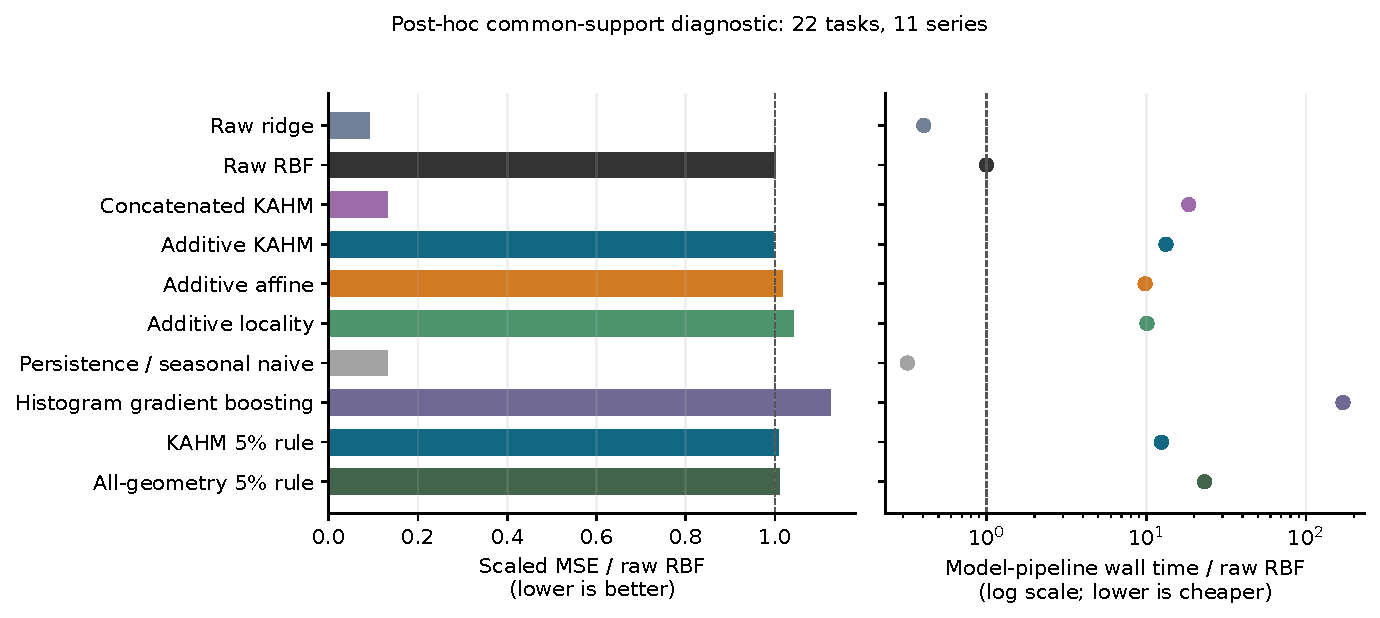
\includegraphics[width=\textwidth]{generated/utility/archive_accuracy_cost.pdf}
\caption{Post-hoc matched-success archive accuracy and cost relative to the raw RBF
procedure. Each ratio uses the equal-source aggregate; individual-source
heterogeneity is retained in Table~\ref{tab:utility-archive-sources}.
The time axis is logarithmic. No confidence interval across windows or
application-wide optimality claim is attached to these four-source
descriptive comparisons.}
\label{fig:utility-accuracy-cost}
\end{figure}
\FloatBarrier

\subsection{Realized residual alignment}
\label{app:utility-residual-results}

For each saved additive forecast, let
$d=\widehat f_{\rm add}(X)-\widehat f_{\rm raw}(X)$, which incorporates
the chosen mixing weight. The prespecified descriptive analysis
reconstructs $2\,\mathrm{mean}\langle Y-\widehat f_{\rm raw}(X),d\rangle$
and $\mathrm{mean}\|d\|^2$ directly from test predictions, averaging
target coordinates and dividing by the fixed training scale for each
archive task in the common-support diagnostic. Their difference equals the realized raw-minus-additive
MSE before rounding. The analysis code and independent manuscript
builder both verify this equality. Table~\ref{tab:utility-residual}
reports the same source hierarchy used for the main loss comparison.

This decomposition describes how the realized correction aligned with
the test residual, including its amplitude cost. It does not identify the
oracle conditional mean in Equation~\eqref{eq:utility-oracle}, explain
which representation component caused the alignment, or supply a new
out-of-sample guarantee. Test-derived terms are never used to retune
the correction, its mixing coefficient, or either adoption policy.

% Generated from the audited forecasting-utility extension; no model fitting.
\begin{table}[!htbp]
\centering\small\setlength{\tabcolsep}{4pt}
\caption{Descriptive test residual decomposition on the post-hoc common-support archive subset. For $d=\widehat f_{\rm add}-\widehat f_{\rm raw}$, alignment is $2\,\mathrm{mean}\langle Y-\widehat f_{\rm raw},d\rangle$ and energy is $\mathrm{mean}\|d\|^2$, averaged over target coordinates and divided by the fixed training scale before hierarchical aggregation. Raw-minus-additive MSE equals alignment minus energy before rounding. These are identities of the saved predictions, not fresh inference or a population certificate.}
\label{tab:utility-residual}
\begin{tabular}{llrrr}
\toprule
Source & Correction & Alignment & Energy & Gain \\
\midrule
Weather & Additive KAHM & -0.0024712 & 0.00068791 & -0.0031591 \\
Weather & Additive affine & 0.00021308 & 0.00097397 & -0.00076088 \\
Weather & Additive locality & -0.0004239 & 0.00036141 & -0.00078531 \\
Solar Weekly & Additive KAHM & 0 & 0 & 0 \\
Solar Weekly & Additive affine & 0 & 0 & 0 \\
Solar Weekly & Additive locality & 0.10669 & 0.059975 & 0.04671 \\
COVID-19 Deaths & Additive KAHM & 0.1667 & 0.045967 & 0.12074 \\
COVID-19 Deaths & Additive affine & -0.59915 & 0.029908 & -0.62906 \\
COVID-19 Deaths & Additive locality & -1.1003 & 0.15312 & -1.2534 \\
Car Parts & Additive KAHM & -0.00065859 & 0.0020919 & -0.0027505 \\
Car Parts & Additive affine & -0.00064528 & 0.0021013 & -0.0027466 \\
Car Parts & Additive locality & -0.058009 & 0.29197 & -0.34998 \\
\midrule
Equal-source mean & Additive KAHM & 0.040893 & 0.012187 & 0.028707 \\
Equal-source mean & Additive affine & -0.1499 & 0.0082457 & -0.15814 \\
Equal-source mean & Additive locality & -0.26301 & 0.12636 & -0.38936 \\
\bottomrule
\end{tabular}
\end{table}

